\documentclass[10pt,a4paper]{article}
\usepackage[latin1]{inputenc}
\usepackage[margin=1in]{geometry}
\usepackage{amsmath}
\usepackage{amsfonts}
\usepackage{amssymb}
\usepackage{graphicx}
\usepackage{float}
\begin{document}
	
\section{Flight Simulation}

To fulfill the requirements of the 2018 IREC Competition, the Texas A\&M University Sounding Rocketry Team (TAMU SRT) must strive to reach an altitude of 10,000 ft AGL with its SRAD Hybrid entry Theseus. In order to meet this metric, the team must have the capability to accurately predict the trajectory of the rocket, given knowledge of the rocket's properties and a realistic assumption of flight conditions. Free, readily available flight simulation software already exists: OpenRocket, a 6 Degree-of-Freedom (6-DOF) software package, and RASAero, a 3-DOF package with advanced aerodynamic analysis, are well respected and used throughout the amateur rocketry community. However, both of these programs are missing key capabilities, such as hybrid engine modeling and advanced atmospheric modeling. Additionally, RASAero only produces nominal flights without any consideration for uncertainty in rocket properties and flight conditions, while OpenRocket accounts for uncertainty but produces only one flight. This creates the need for a flexible, easily extensible flight simulation that can quantify the uncertainty in a trajectory through the Monte Carlo method. The SRT Flight Sim (SRT FS), a 3-DOF simulation suite implemented in MATLAB\textregistered, has been developed to fulfill this need.


\subsection{Methodology}

\subsubsection{Overview}

The SRT FS operates within a 3-DOF model with translation in the x and z directions as well as rotation about the y direction. The translational equation of motion is shown in Eq. \ref{eq:translation} where $\vec{x}$ is the position vector of the rocket and $\vec{T}$, $\vec{L}$, $\vec{W}$, and $\vec{N}$ are the thrust, lift, weight, and normal force vectors, respectively. 

\begin{equation}
\frac{d^2}{dt^2}\vec{x} = \frac{\vec{T}+\vec{L}+\vec{W}+\vec{N}}{m}
\label{eq:translation}
\end{equation}

The rotational equation of motion in the x-z plane about the time varying center of gravity is shown in Eq. \ref{eq:rotation} where $\theta$ is the pitch attitude angle and where $M_A$ and $M_D$ are the moments due to aerodynamic forces and pitch damping. Also, $I_{yy}$ represents the rocket's moment of inertia about the y-axis.

\begin{equation}
\frac{d^2}{dt^2}\theta = \frac{M_A+M_D}{I_{yy}}
\label{eq:rotation}
\end{equation}

\begin{figure}[h!]
	\centering
	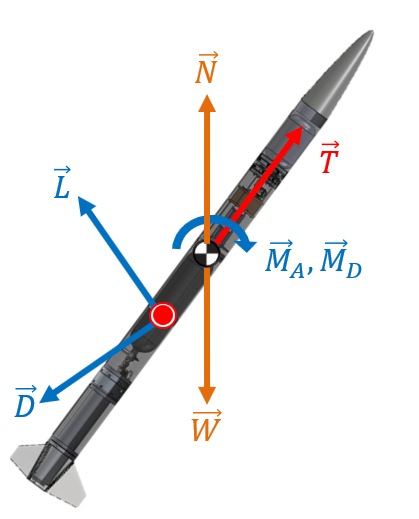
\includegraphics[width=.3\textwidth]{./figs/rocket_force.png}
	\caption{Forces of Rocket Flight}
	\label{fig:rocket_force}
\end{figure}


These forces and moments are shown acting upon the rocket body in Figure \ref{fig:rocket_force}. The Runge-Kutta-Fehlberg Method (RKF45) is used to numerically solve these differential equations of motion. At every time step, random error is inserted into rocket and atmospheric properties; the random error is derived from Uniform, Gaussian (Normal), or Wiener distributions with parameters ($\mu$, $\sigma$, etc.) chosen appropriately for variables such as ambient temperature, wind velocity, humidity, etc..

All input quantities are defined by the user in a C/C++ style text document. This file contains all weather conditions, all vehicle and engine properties, simulation properties (time-step, number of Monte Carlo, etc.) as well as a directory to the aerodynamic data used (obtained from RASAero). This input method was chosen in such a way as to be easily scriptable allowing the SRT FS to have further applications such as input sensitivity studies and flight performance envelopes.

The program is run through the main function, where the user chooses the text based input file they wish to analyze. At this point the input function is parsed and all variables and statistical distributions are loaded into the model. The FS then randomizes the relevant variables with their associated distribution. An atmospheric model is then built using the Standard Atmosphere assumptions for isothermal and gradient regions, up to ~280,000 ft above sea level (ASL); this model takes in launch site temperature, pressure, humidity, and elevation, and outputs temperature, pressure, and density as a function of altitude. Using the dry lapse rate of each atmospheric region, the partial pressure of water vapor is found as a function of altitude, and a density correction for humidity is applied. Propulsion data is then input into the SRT Hybrid Engine Model and the appropriate thrust curve and engine mass data is retrieved. A calculation function in conjunction with the main function perform the RKF45 numeric integration and calculate the rocket state for each time-step until the specified time of flight has been reached. All time histories of each flight are stored in their own file. The user may now choose to use an additional post-processing function which will plot and compile statistics of the flight data. A flow-chart of the FS program is given in the following figure.
\begin{figure}[h!]
	\centering
	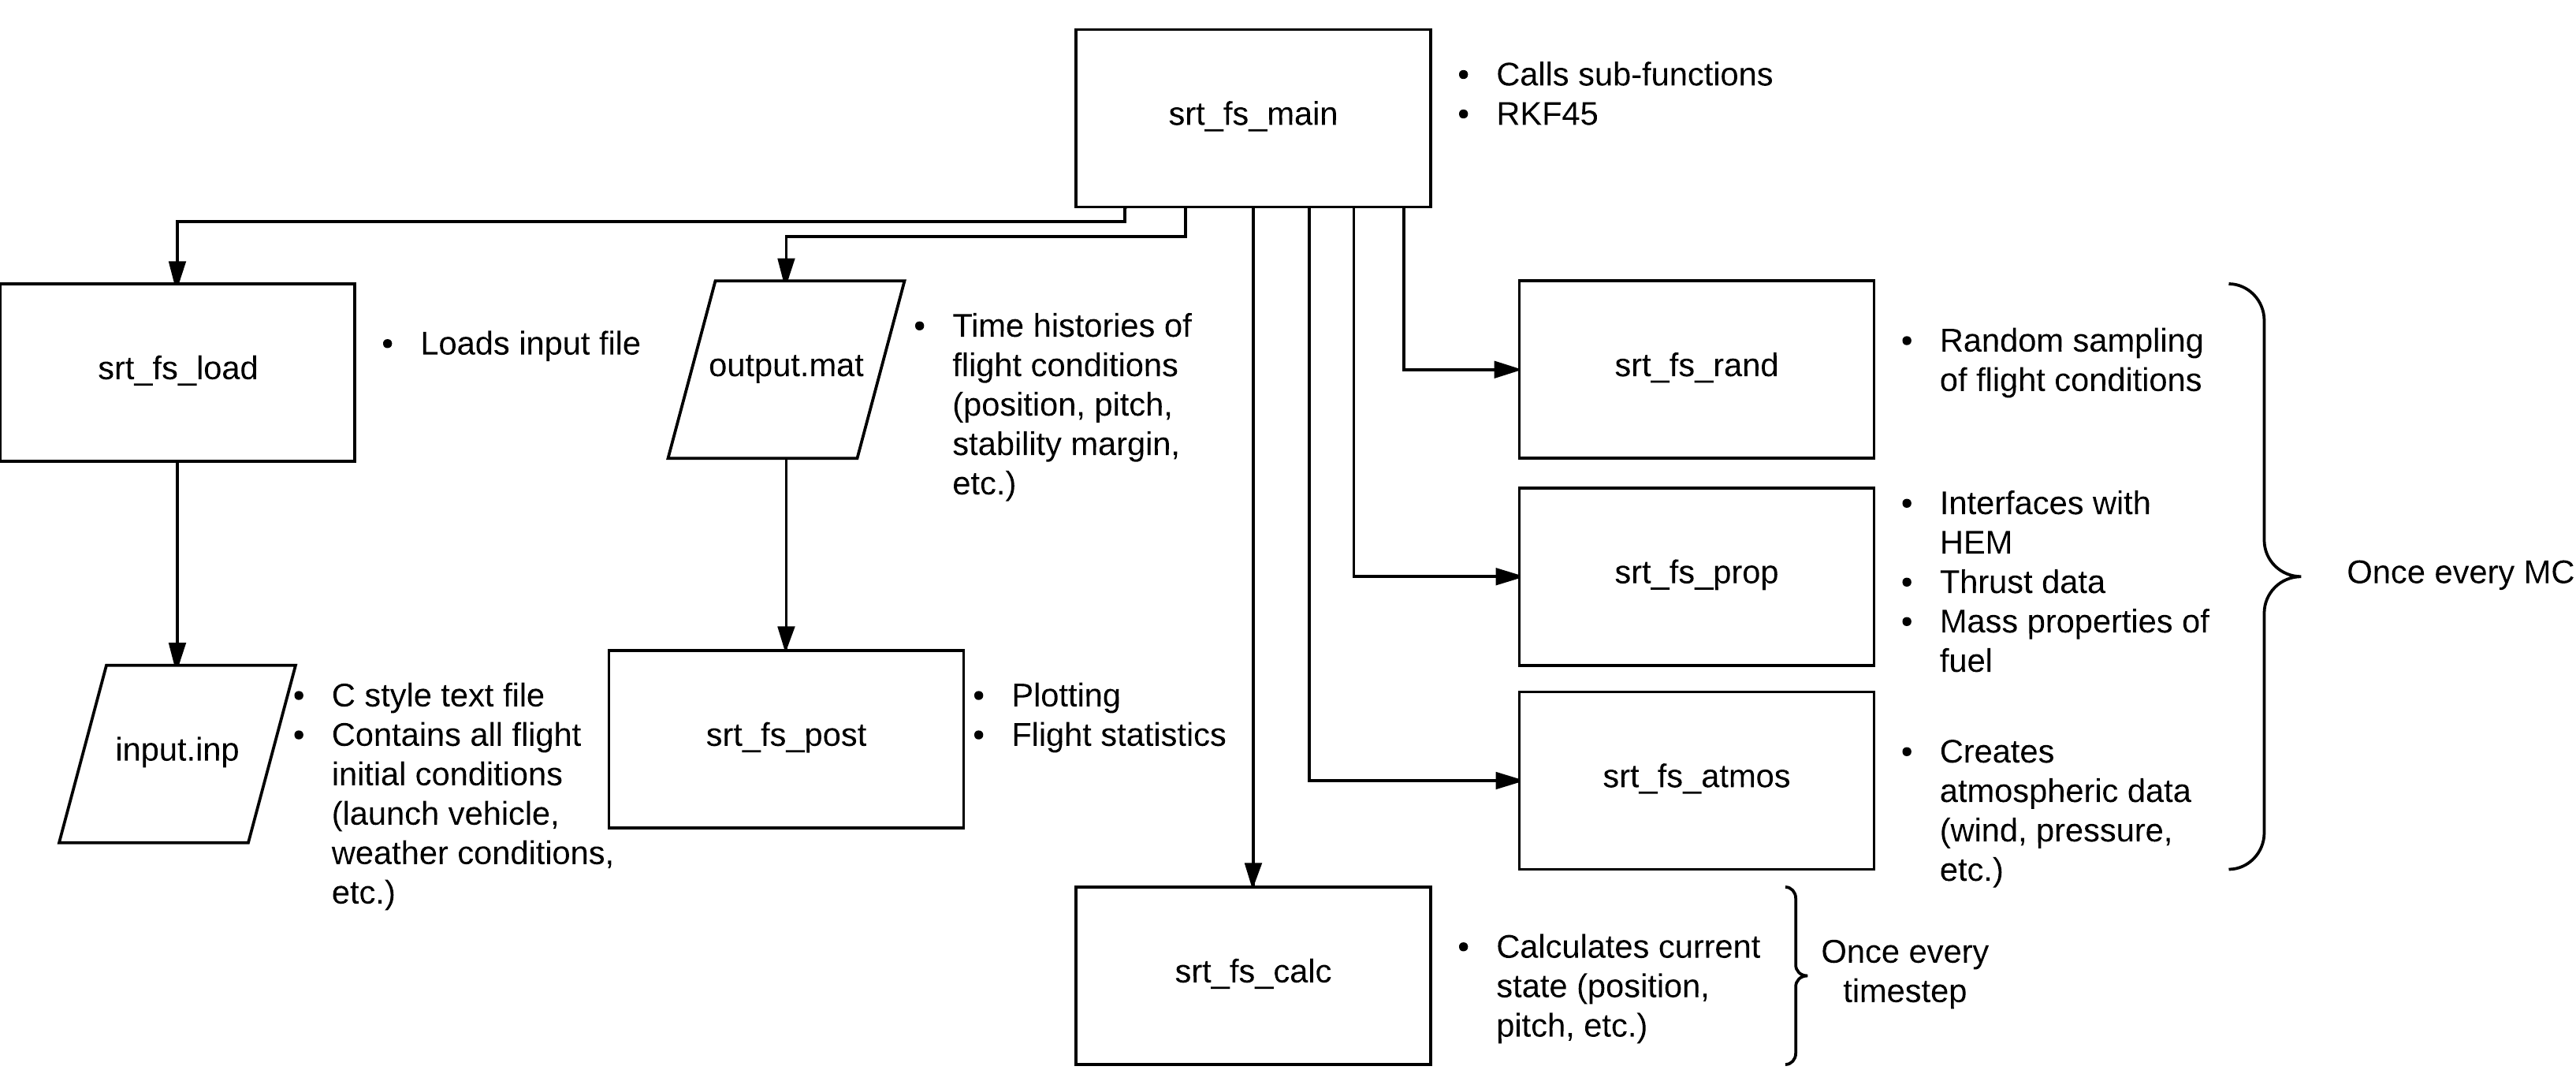
\includegraphics[width=1.05\textwidth]{./figs/fs_flow.png}
	\caption{SRT Flight Sim Operation}
	\label{fig:fs_flow}
\end{figure}


\subsubsection{Monte Carlo Method}


\begin{figure}[H]
	\centering
	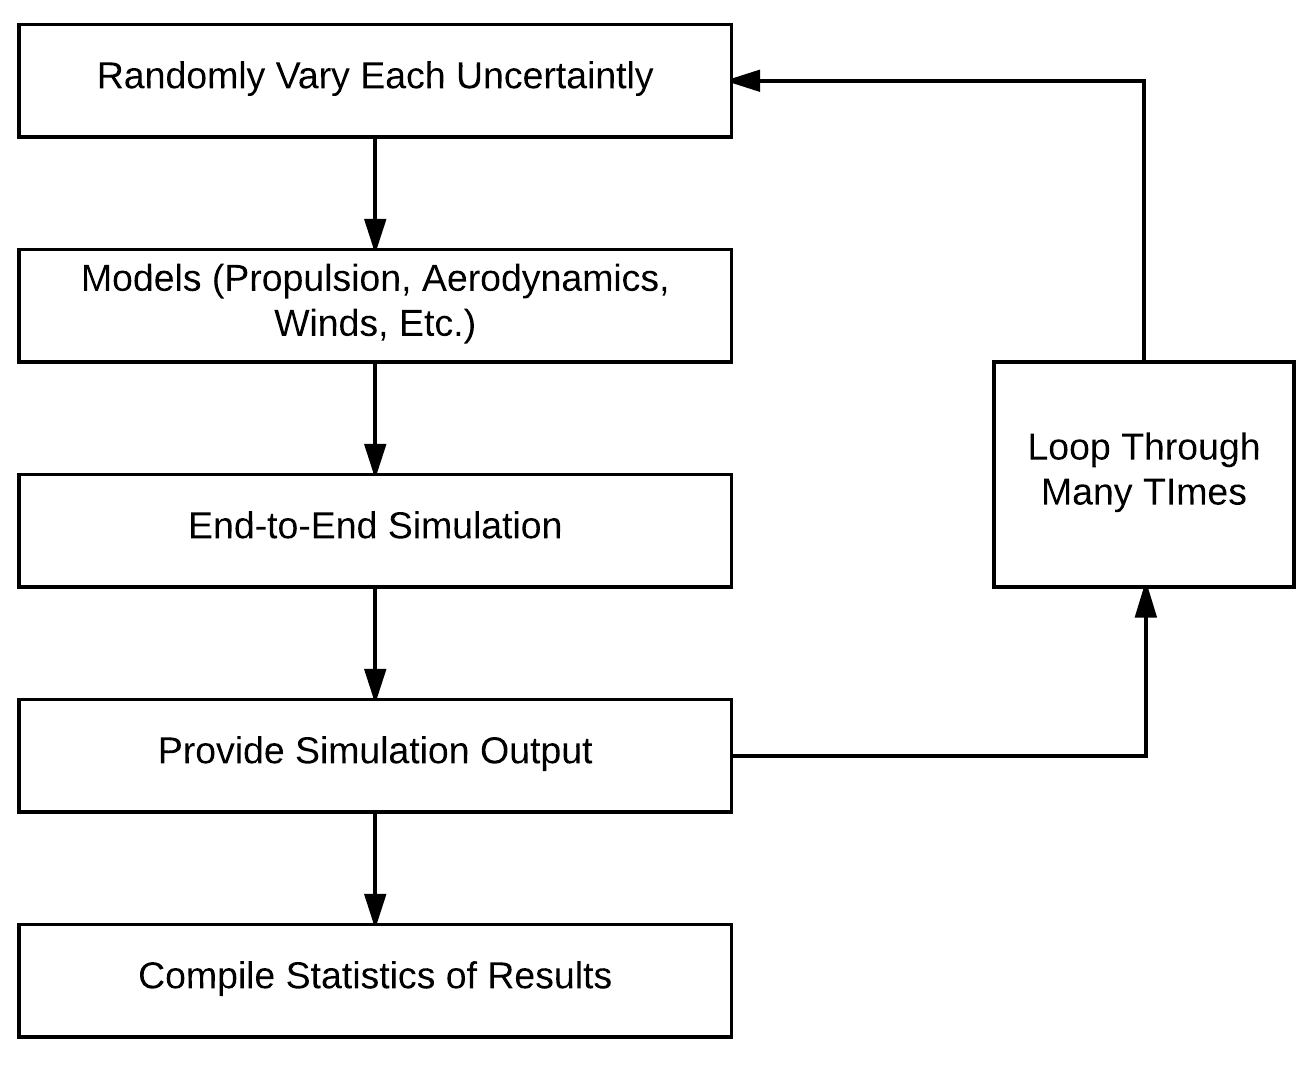
\includegraphics[width=.6\textwidth]{./figs/monte_carlo_process.png}
	\caption{Monte Carlo Process}
	\label{fig:monte_carlo_process}
\end{figure}
It is natural to have a degree of uncertainty in launch conditions for any given flight. For example, the exact weather conditions on the day of a launch are likely to be known only within a range of values. The Monte Carlo method of flight simulation aims to deal with these uncertainties through means of statistical analysis of many different flight simulations \cite{monte_carlo}. Each of these simulations uses a different random sample of input conditions within a specified range or distribution. By simulating many flights over a spectrum of input conditions, a spread of possible flight outputs can be obtained (Figure \ref{fig:flight_spread}). For the rocket's ascent, the time history of every flight variable (position, velocity, acceleration, etc.) is processed across the entire set of random flights, yielding a mean behavior. This mean behavior, in addition to the standard deviation and maximum/minimum values associated with each variable, allows the user to make quantitative assessments about the uncertainty in the nominal trajectory. It is important to note that for each flight the input sampling algorithm is fed a user defined random number seed which is specified in the simulation inputs. This seed control allows for accurate comparison over different simulations. 

\begin{figure}[H]
	\centering
	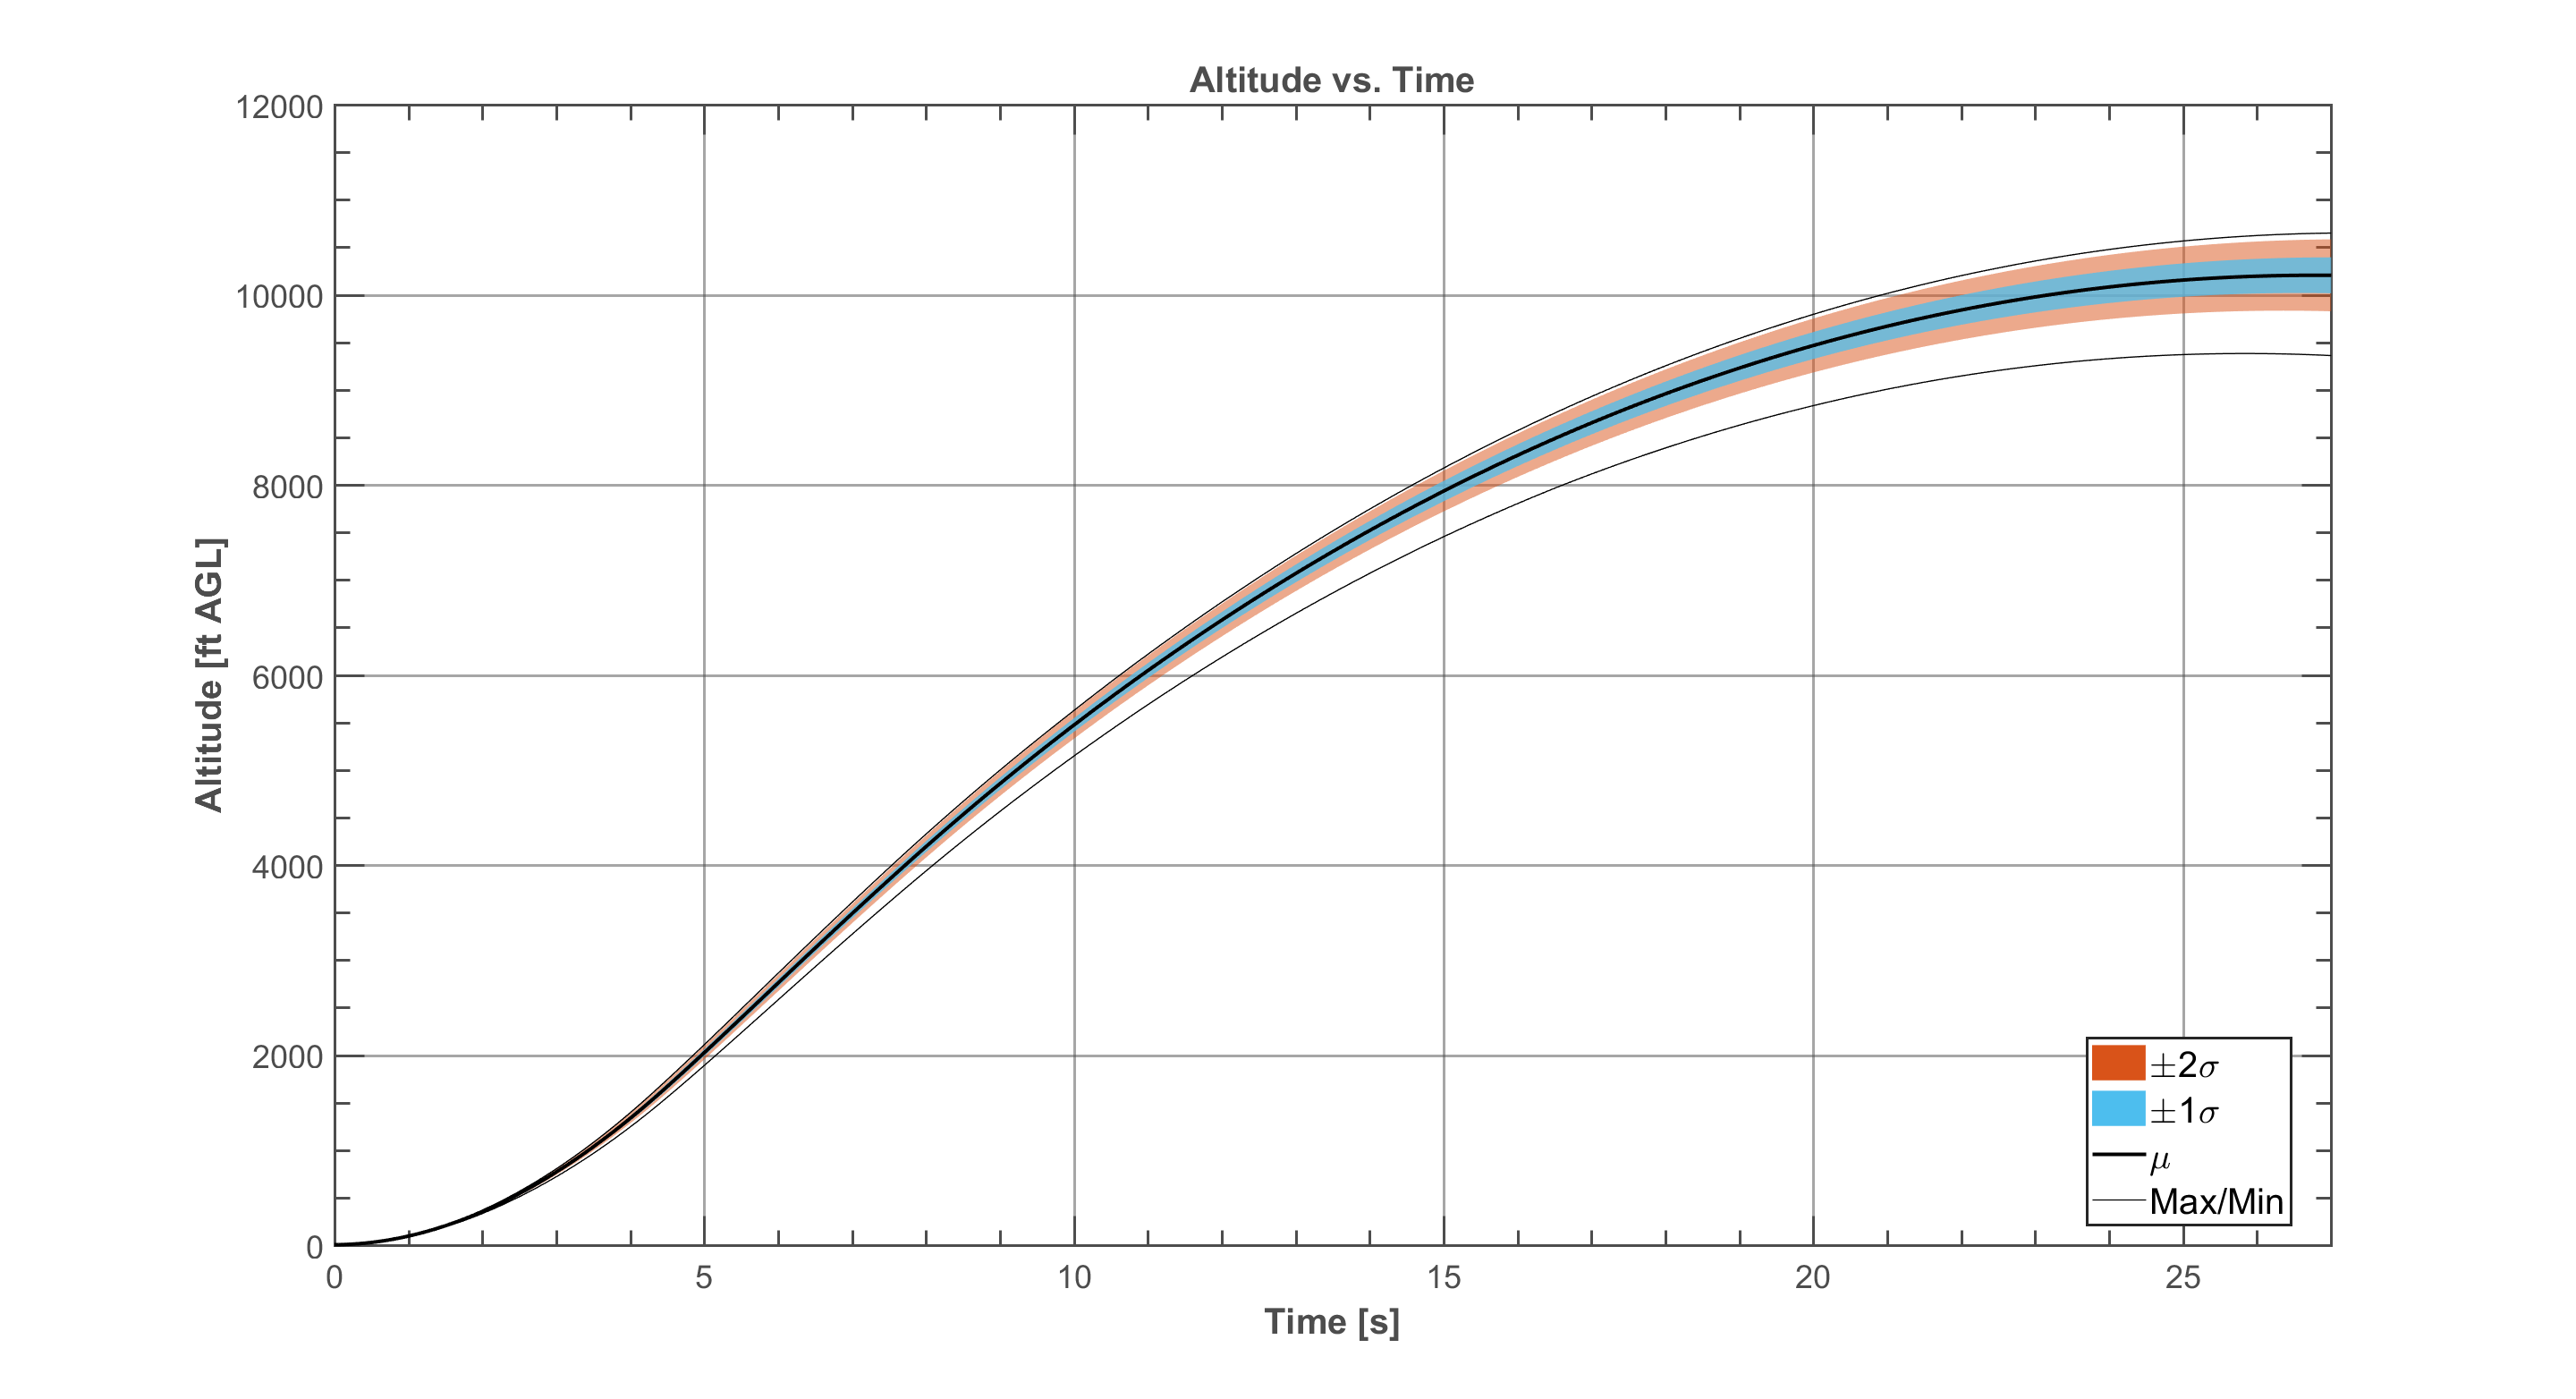
\includegraphics[width=.9\textwidth]{./figs/flight_spread.png}
	\caption{1000 Monte Carlo Altitude Spread}
	\label{fig:flight_spread}
\end{figure}


\subsubsection{Variable Distributions}
%%Atmospheric properties

A stochastic wind model using the Dryden form (Eq. \ref{eq:dryden}) of the power spectral density function (a description of the power contained within a specific frequency) for turbulence magnitude is used to model atmospheric turbulence \cite{dryden}. This model produces a "frozen" turbulence which is a function of position alone.


\begin{equation}
\Phi_u (\Omega) = \sigma_u^2 \frac{2L_u}{\pi}\frac{1}{1+(L_u\Omega)^2}
\label{eq:dryden}
\end{equation}
The value of the scale length is given as: $L_u = 1750$ ft and $\sigma_u$ is the standard deviation of the lateral wind velocity.

To extract wind velocities from the above expressions the sum of sinusoids method is used. The power spectral density function is first parceled into N equal sections in such a way that each section contains an equal area. The area of each section is denoted by:
\begin{equation}
A_u =\sigma_u\sqrt{2/N}
\end{equation}
The frequency of this function is unbounded; therefore, an arbitrarily large frequency is chosen as the upper bound for integration and the function is subdivided within these bounds. Justification for this cutoff frequency can be seen by a simple inspection of the power spectral function, which indicates the overwhelming majority of the power lies within the low frequencies, and thus disregarding the highest frequencies will not substantially alter the resulting wind function. An example of such parceling is shown in Figure \ref{fig:dryden} where the Dryden spectra is divided into 25 sections and the cutoff frequency is chosen as 1 [rad\textbackslash ft]. Each spatial frequency value derived through this method is used as the frequency for an individual sine function.

\begin{figure}[h!]
	\centering
	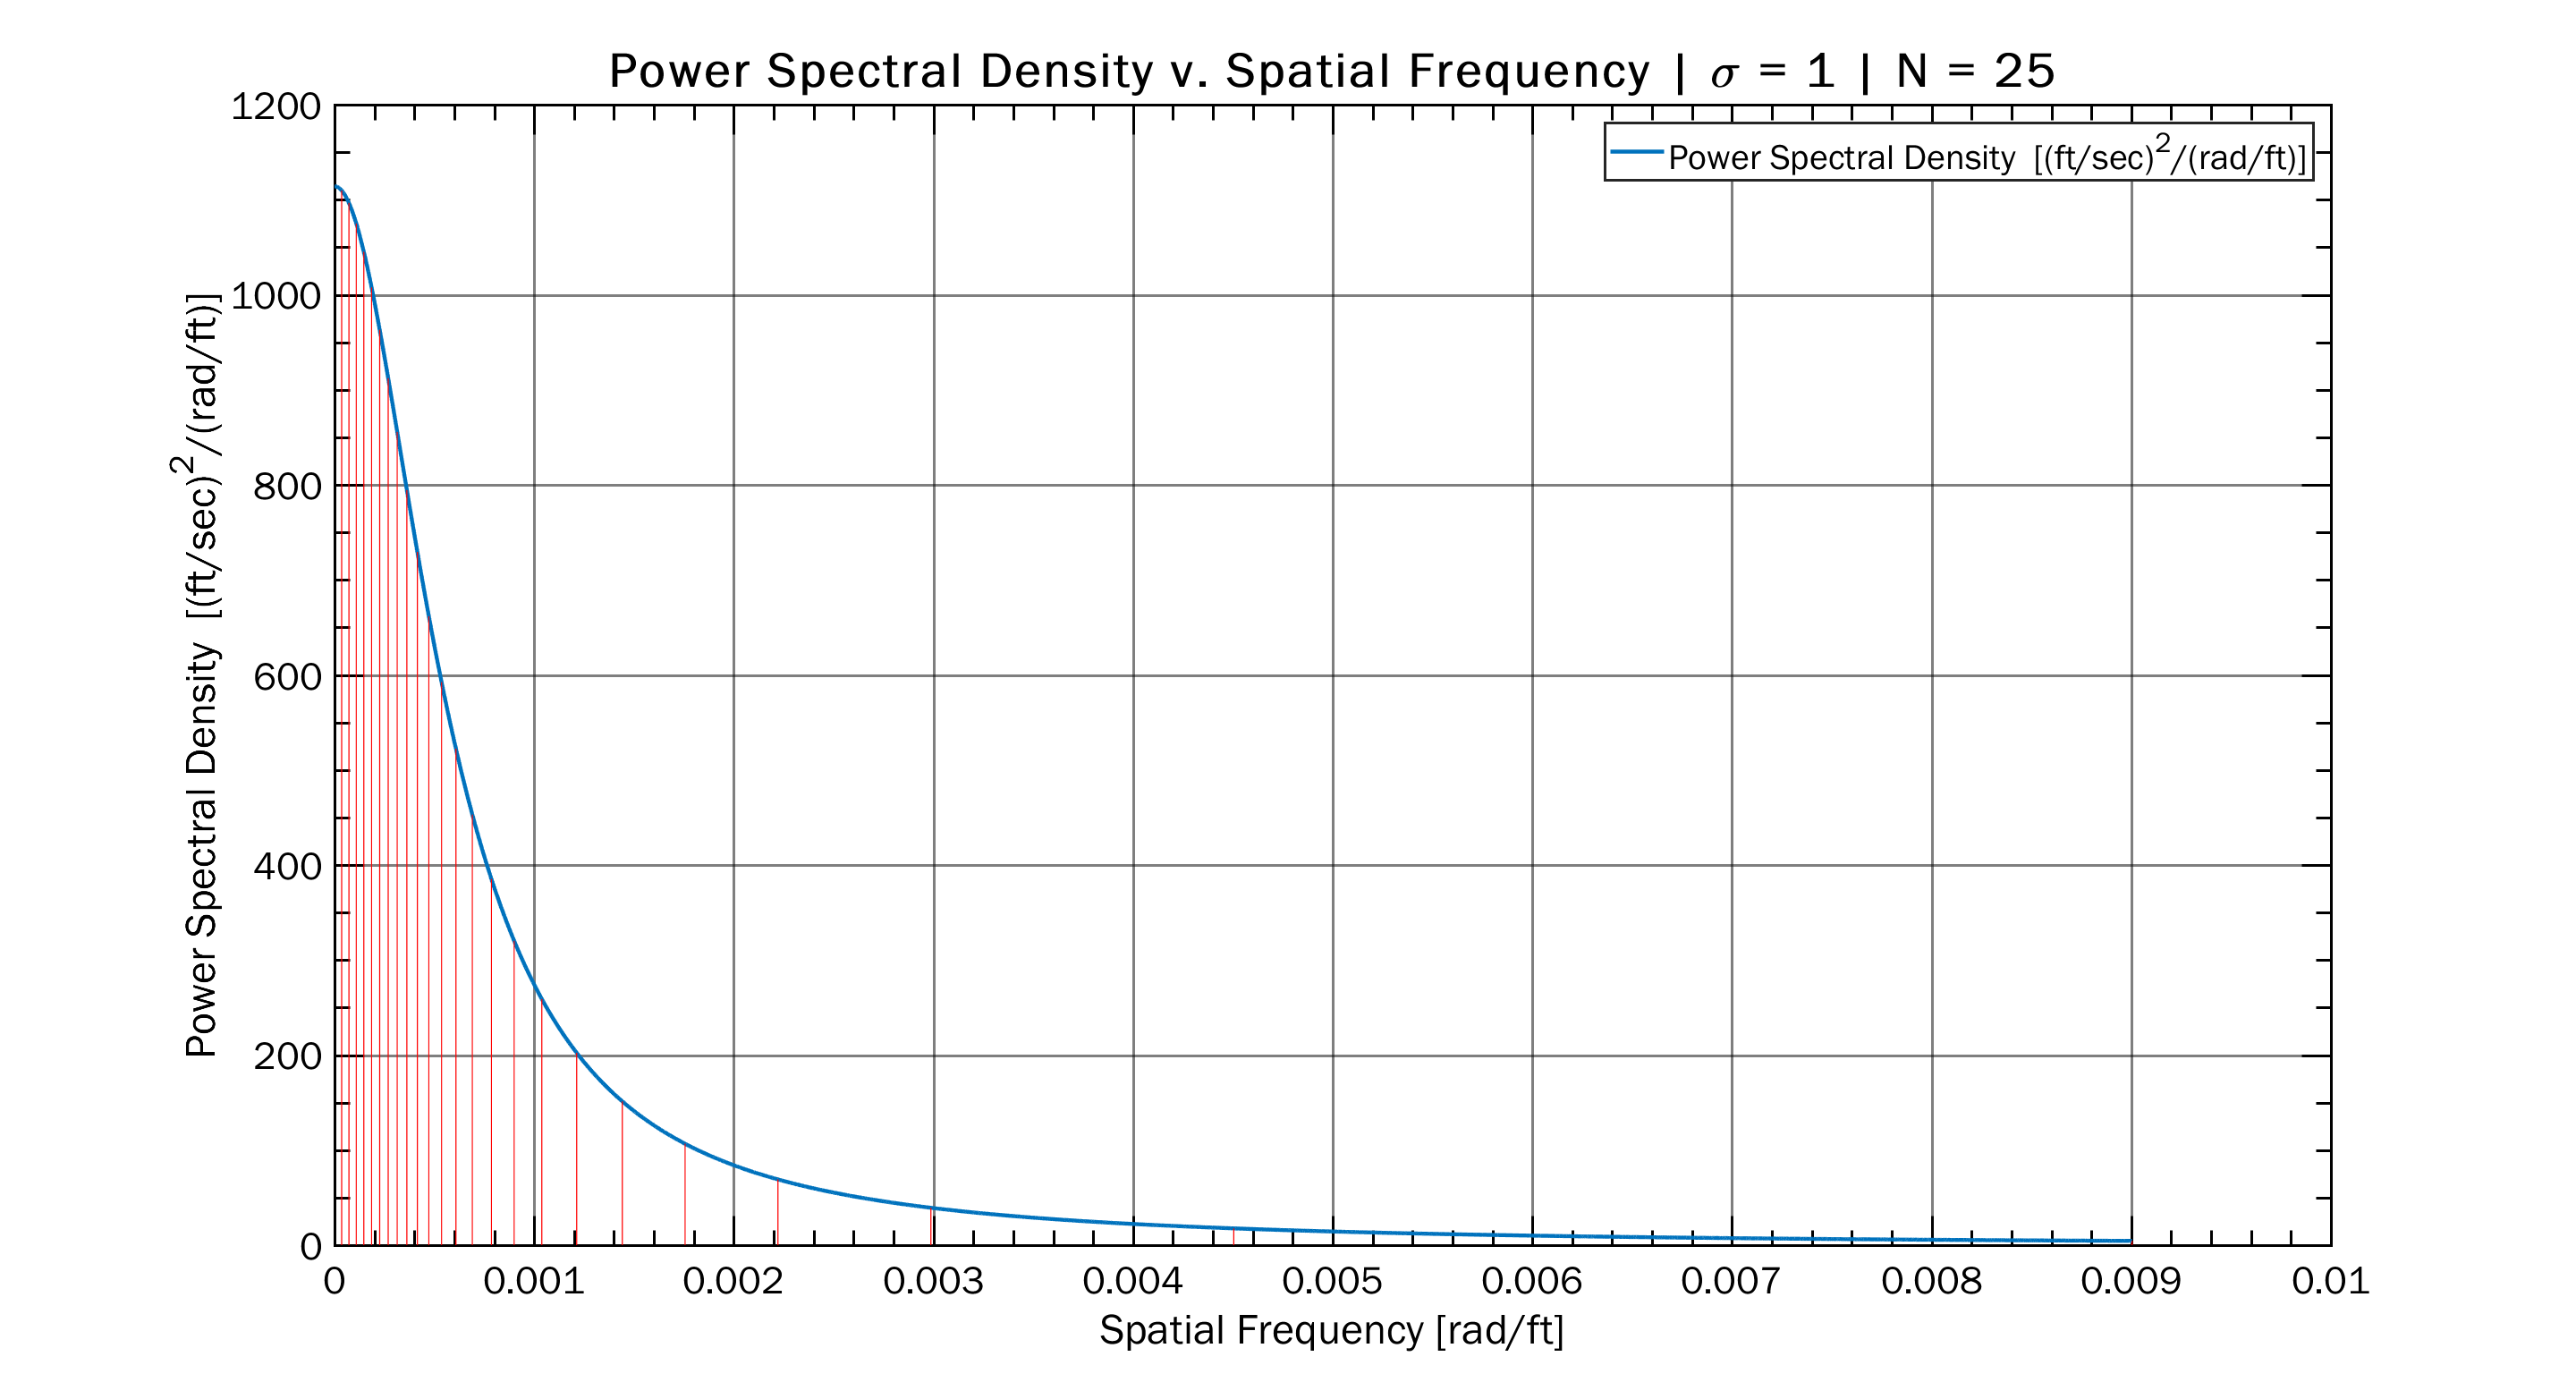
\includegraphics[width=1\textwidth]{./figs/dryden.png}
	\caption{Spectral Power Density}
	\label{fig:dryden}
\end{figure}
The wind velocity at any downrange position is given by a summation of these sin functions is expressed as:
\begin{equation}
u(x) = A_u\sum _{i=1}^{n}\sin[(\Omega_u)_ix+(\epsilon_u)_i]
\label{eq:wind_vel}
\end{equation}


Where, $\epsilon_u$ is a random phase shift of each sin wave. This phase shift is sampled uniformly on the distribution of $-\pi$ to $\pi$ and utilizes the random seed from the simulation input. 
\begin{figure}[h!]
	\centering
	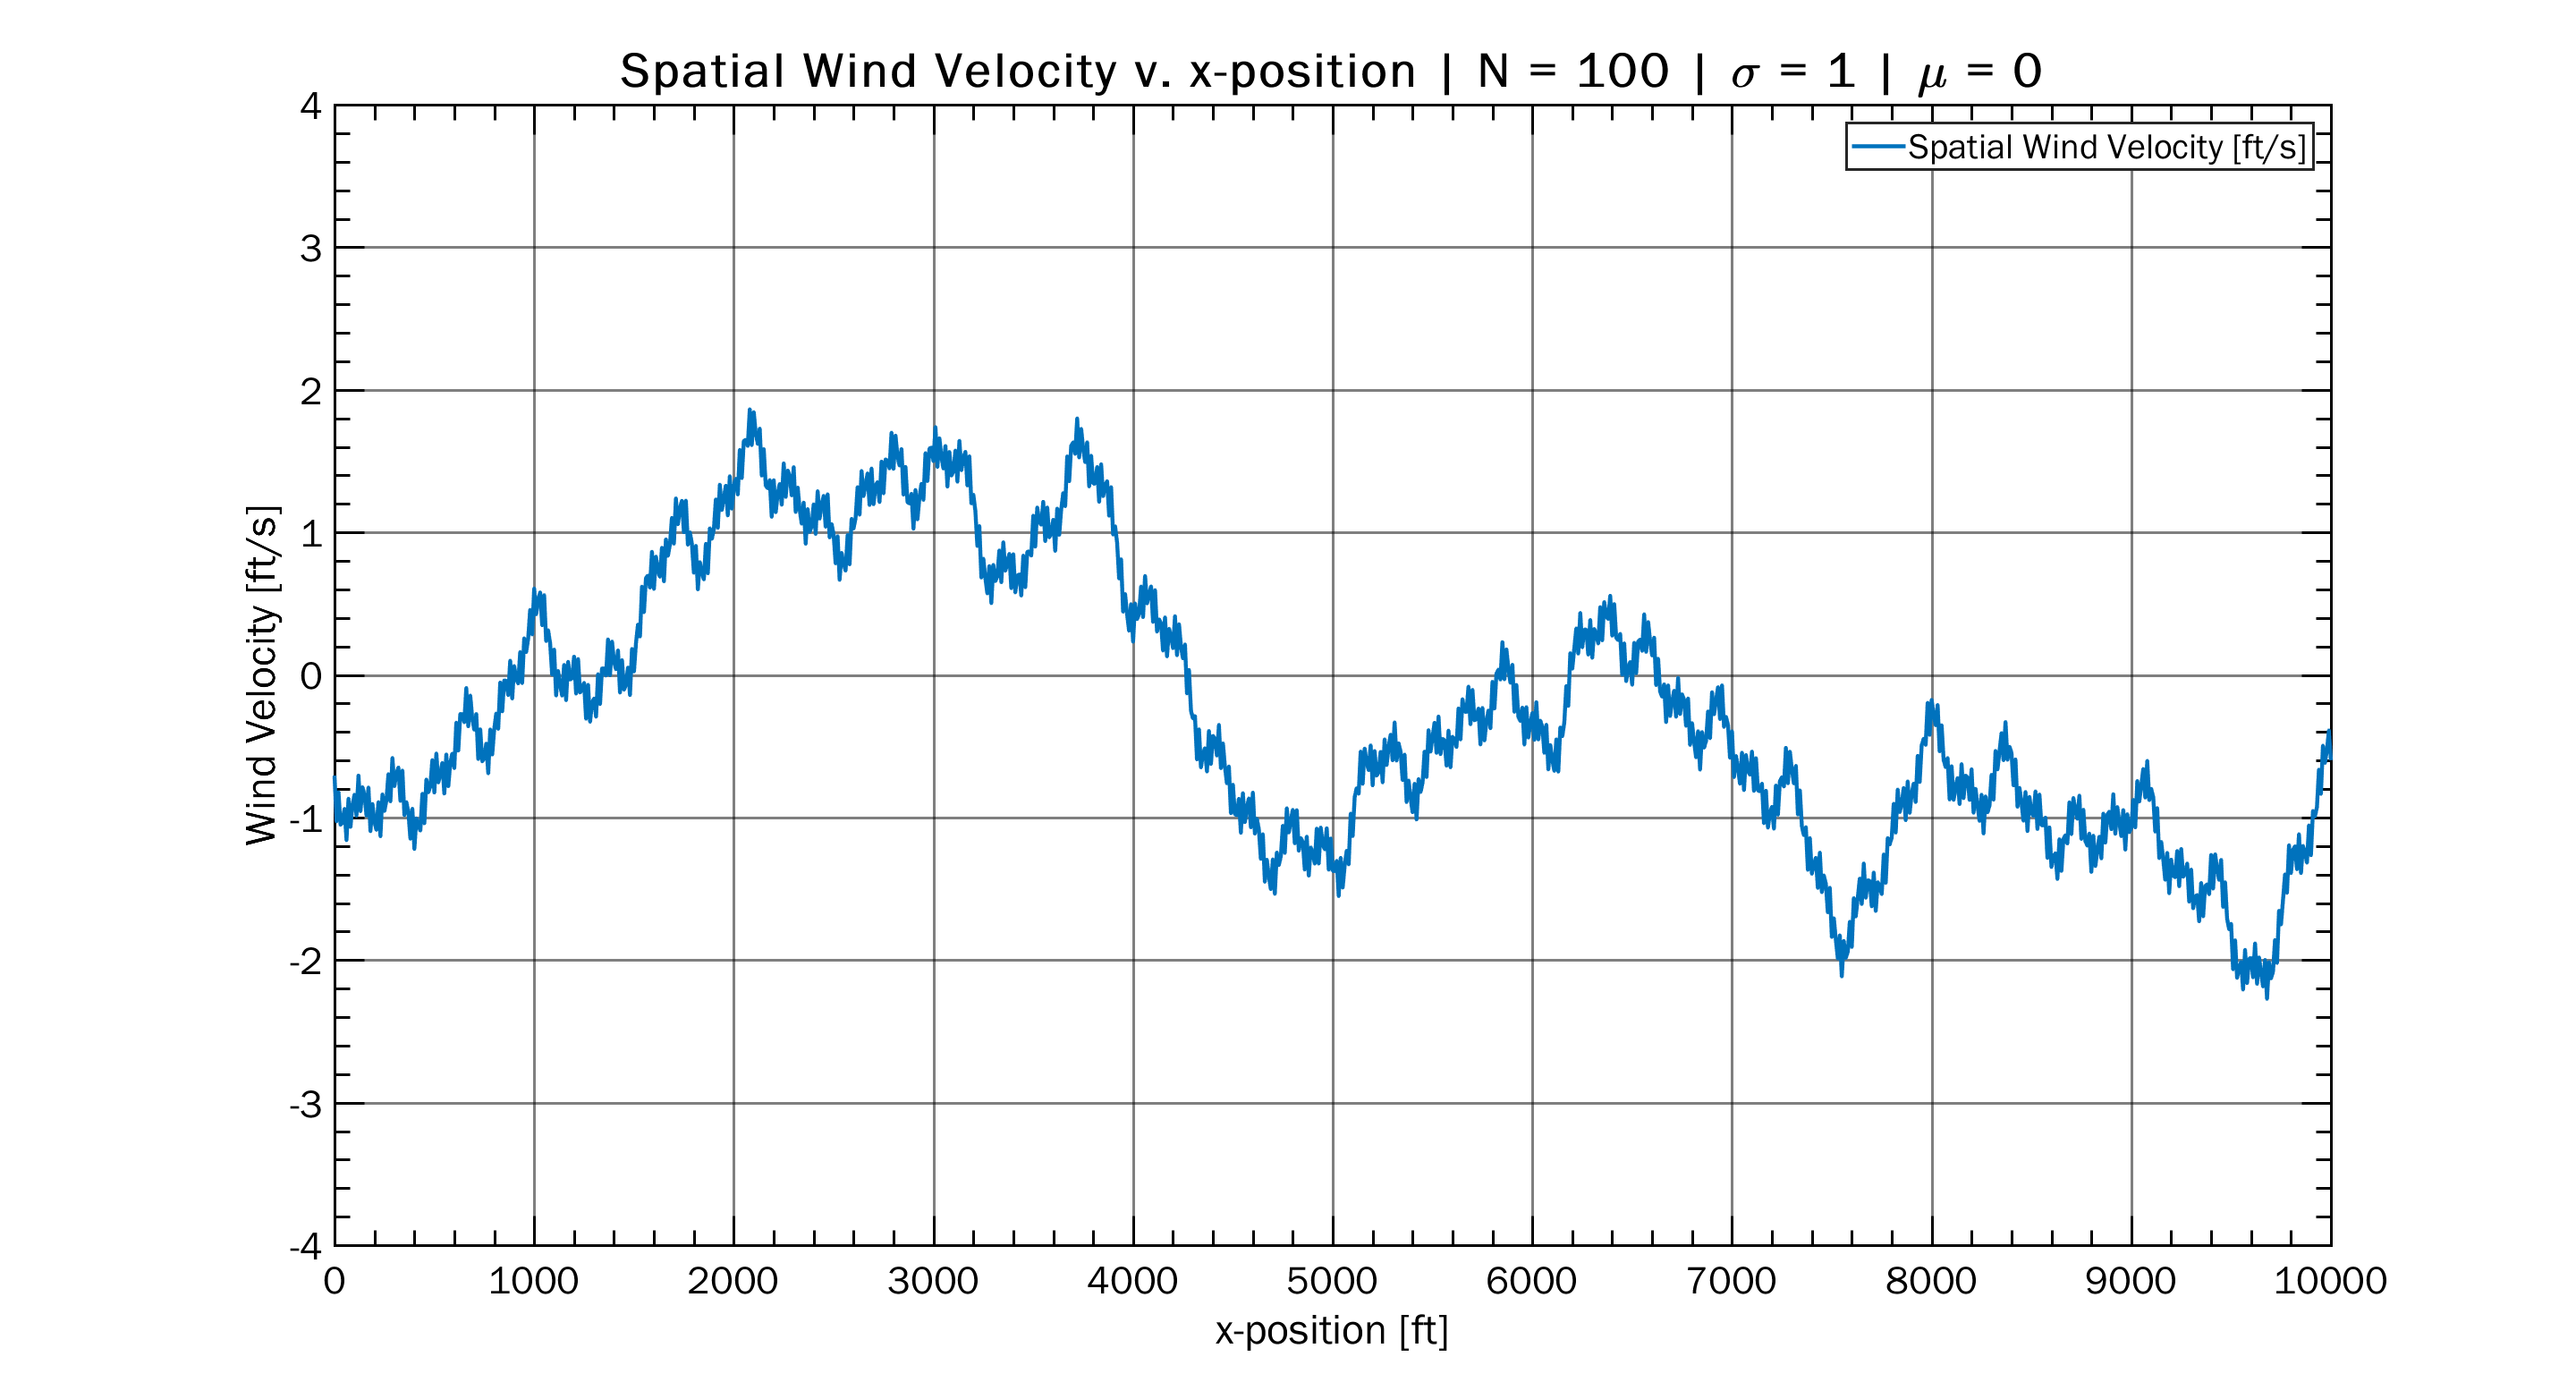
\includegraphics[width=1\textwidth]{./figs/wind.png}
	\caption{Spatial Wind Magnitude}
	\label{fig:wind}
\end{figure}

\subsection{Flight Performance Envelopes}

The Monte Carlo method allows for a more accurate characterization of flight performance across a large range of input conditions. A Flight Performance Envelope (FPE) allows for a characterization of vehicle performance over a range of two independent variables. An example FPE is shown in Figure \ref{fig:apogee_eta70} in which apogee is characterized over the parameters of dry mass and nitrous fill. 
\begin{figure}[H]
	\centering
	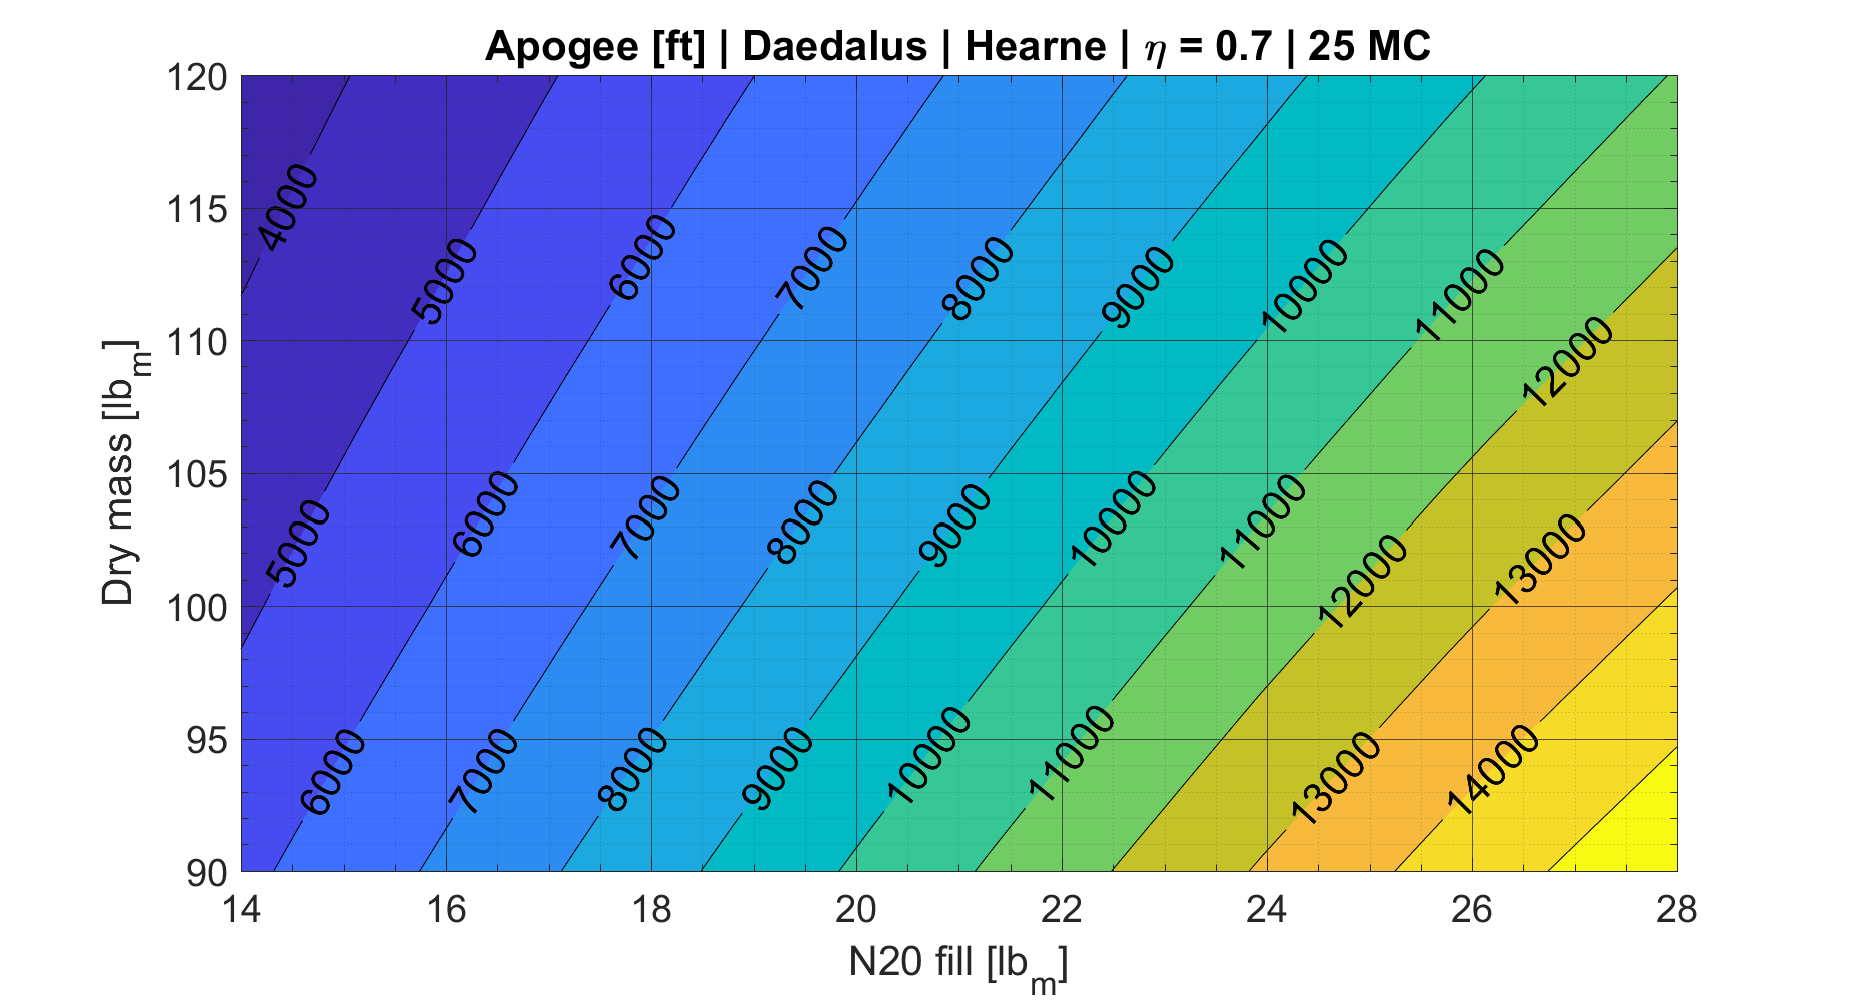
\includegraphics[width=1\textwidth]{./figs/apogee_eta70.png}
	\caption{Apogee Characterization}
	\label{fig:apogee_eta70}
\end{figure}

For every grid point seen a number of flights are run, in the example shown 25 MC are performed within each grid point, which provides a greater justification to the accuracy of this method. Contours are then drawn along regions of equal value. 

FPEs provide a useful method of determining the design parameters required for desired performance characteristic, as one can simply look up the desired flight condition and find which combination of input parameters provide the desired output. FPEs are also useful as a tool in determining launch safety, particularly in a safety analysis at rail exit. Figure \ref{fig:rail_exit} shows a characterization of rail exit velocity based on nitrous fill and tank temperature. On the day of launch these values will be known with a high degree of precision and thus one will be able to quickly determine an estimate of rail exit velocity. This figure also is useful for determining nitrous overfill conditions (marked in red). The National Association of Rocketry recommends a rail exit velocity at least four times greater than the lateral wind speed \cite{nar}. A simple check that rail exit velocity is four times greater than the lateral wind speed measured is a first step in determining launch safety.
\begin{figure}[h!]
	\centering
	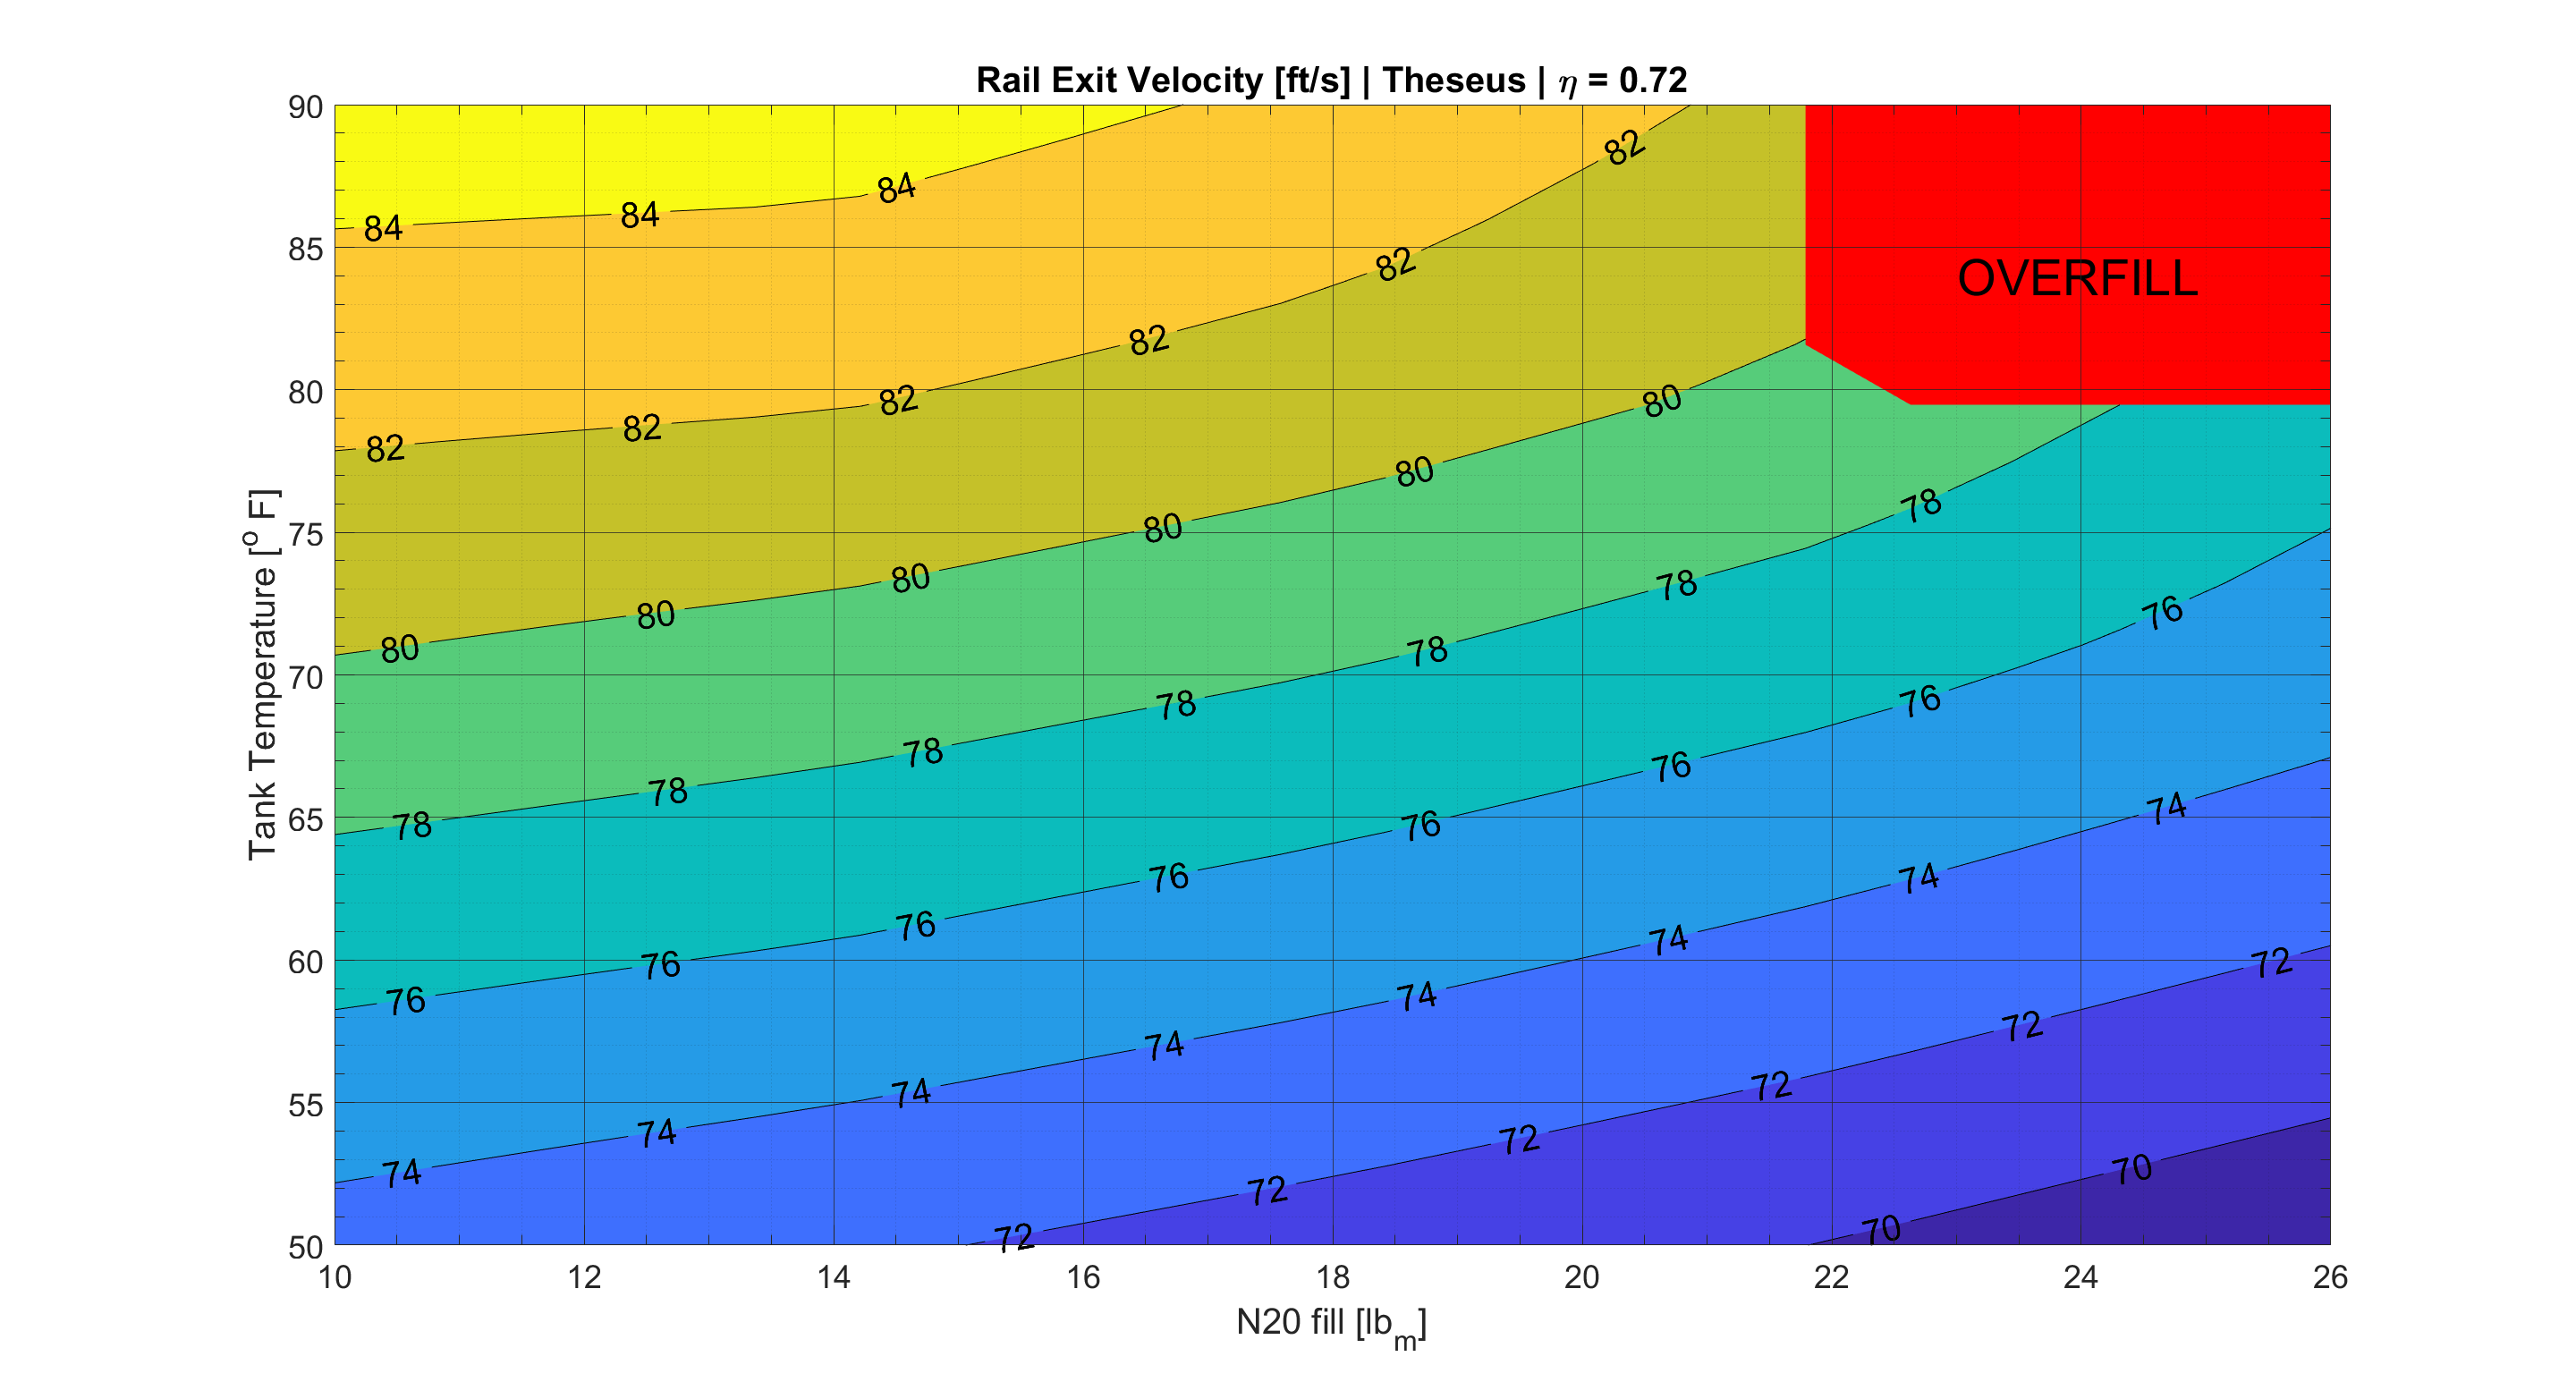
\includegraphics[width=1\textwidth]{./figs/rail_exit.png}
	\caption{Rail Exit Velocity}
	\label{fig:rail_exit}
\end{figure}

 Vehicle specific safety measures beyond a general rule of thumb are also required; thus an analysis of stability margin at rail exit is also required. Figure \ref{fig:stab_50} shows the relationship between nitrous fill, lateral wind velocity, and minimum stability margin experienced at rail exit with a tank temperature of 50 $^o$ F. This provides further information as to the stability of the rocket at rail exit and provides more information to those determining if a launch is within the margin of safety desired. Areas with a minimum stability margin of less than 0.75 [cal] are marked with red as this has been determined to be beyond the range of acceptable safety.
 \begin{figure}[H]
 	\centering
 	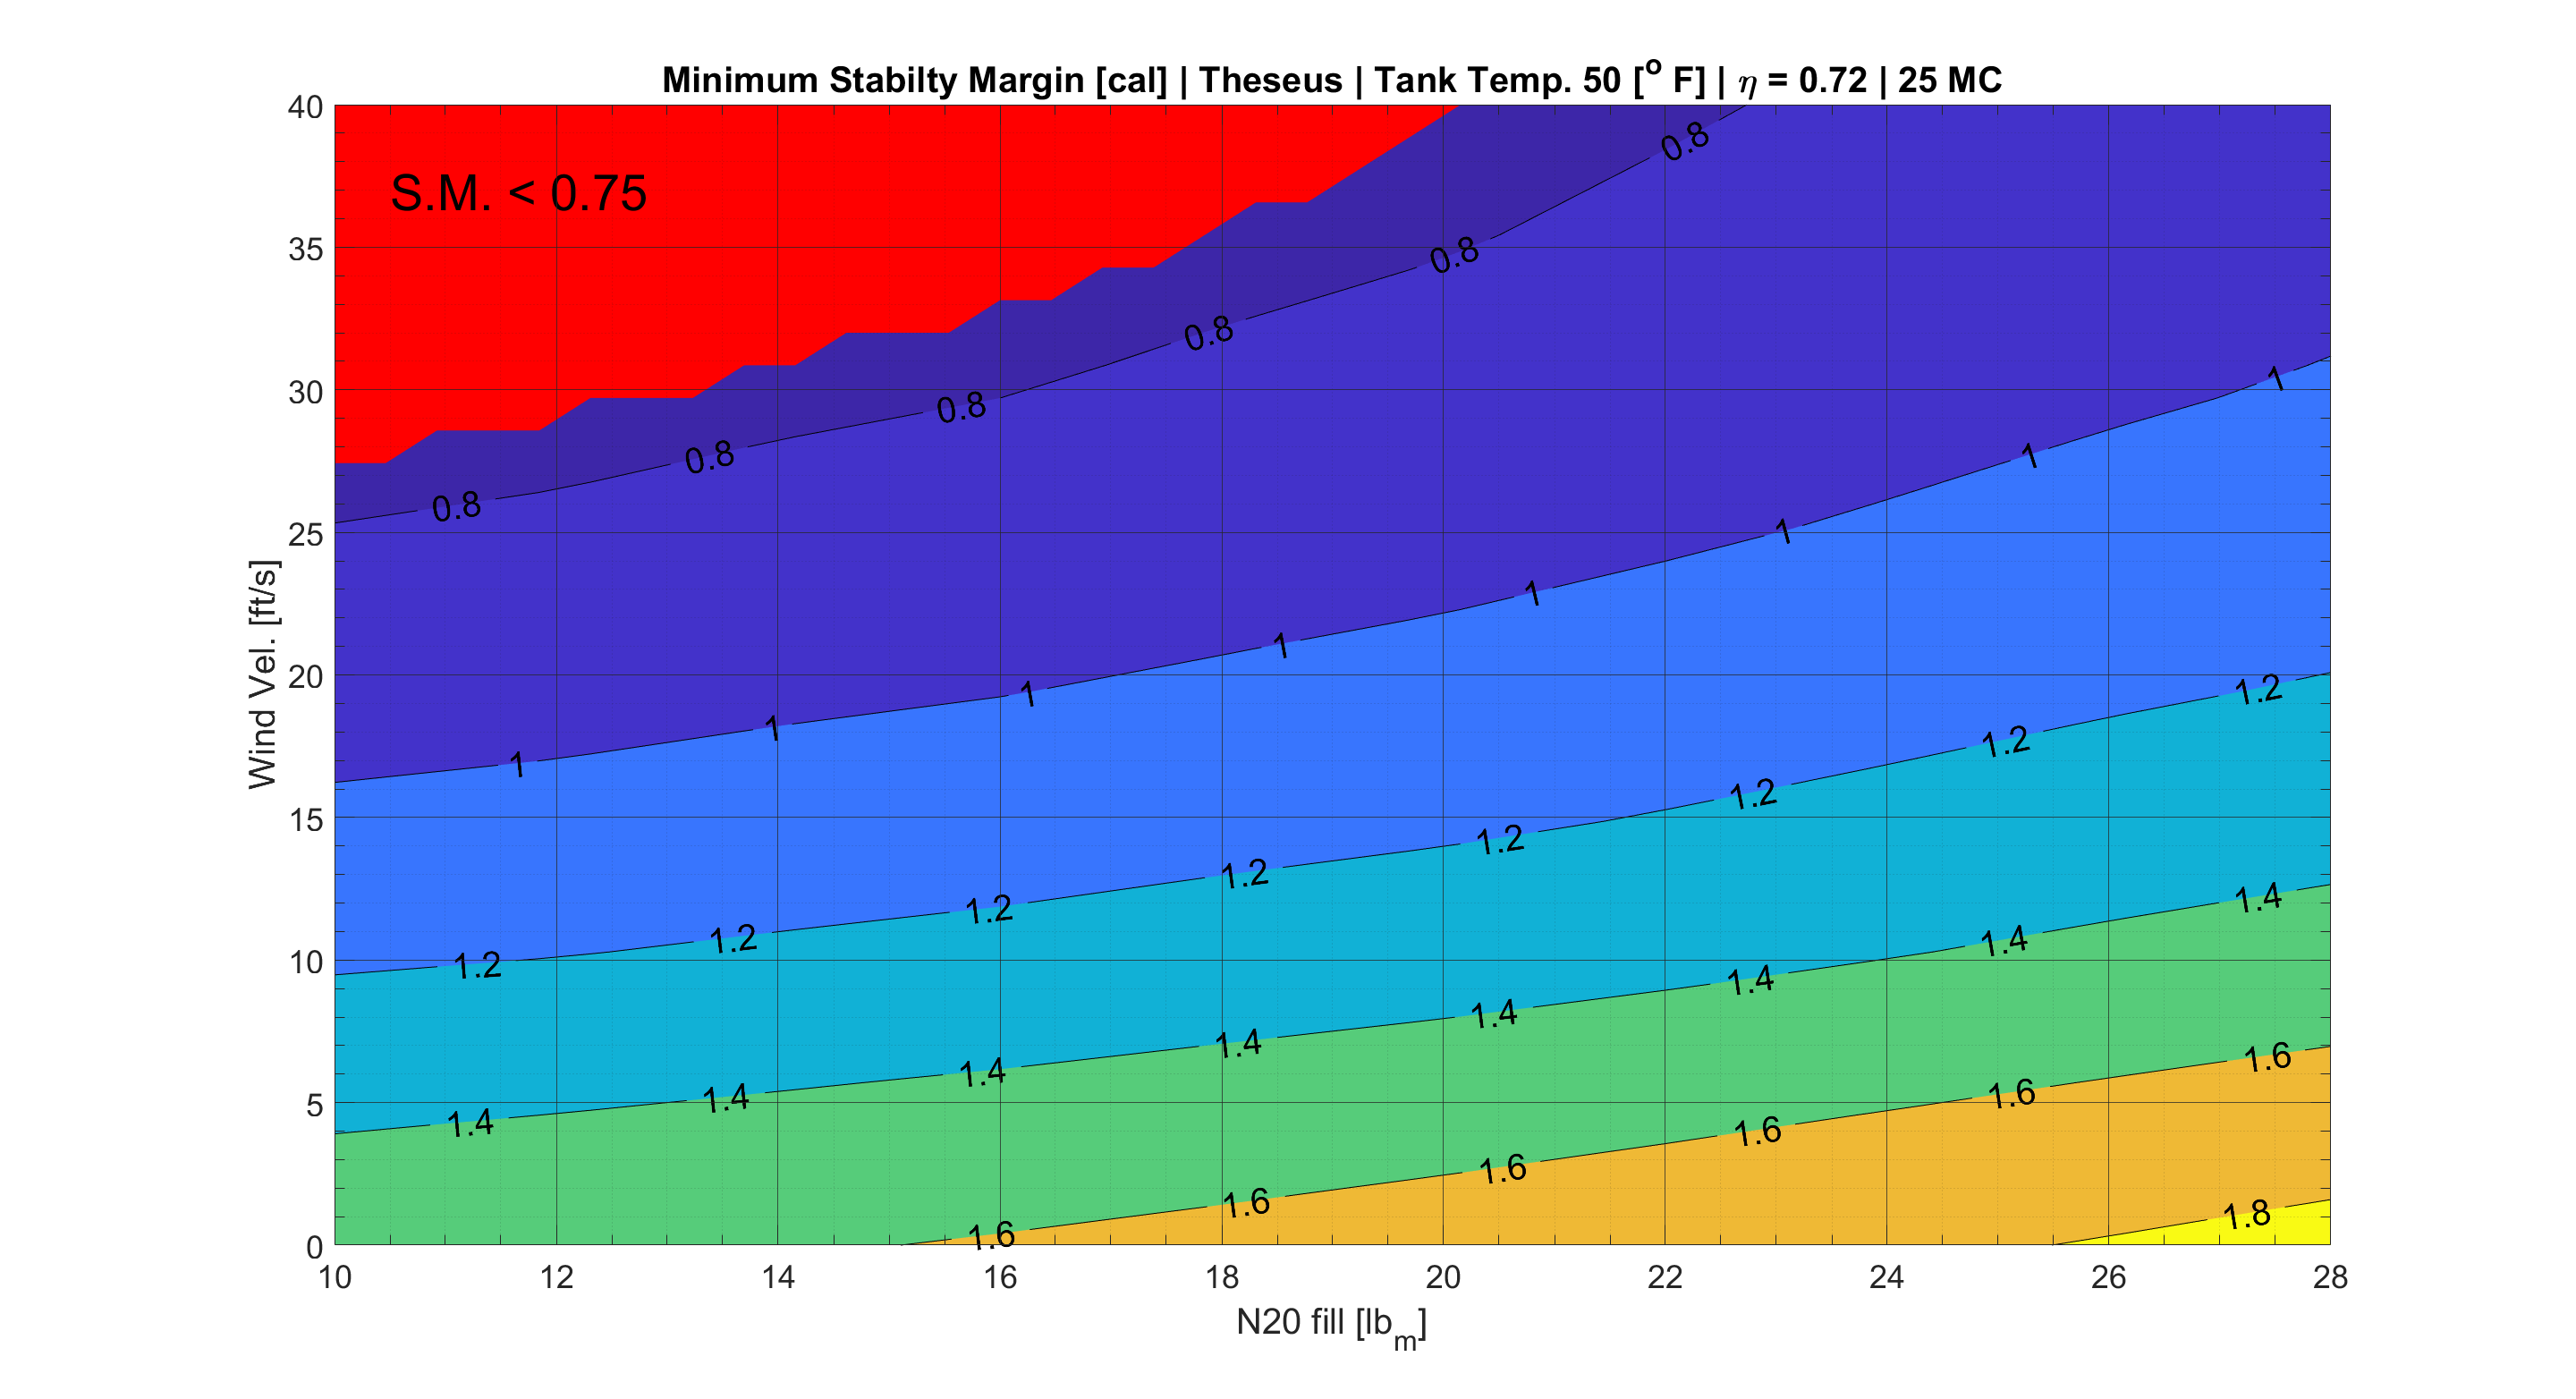
\includegraphics[width=1\textwidth]{./figs/stab_50.png}
 	\caption{Minimum Stability Margin at 50 $^o$ F}
 	\label{fig:stab_50}
 \end{figure}
 
 Figure \ref{fig:stab_70} and \ref{fig:stab_90} show the same relationship for a tank temperature of 70 $^o$ F and 90 $^o$ F, respectively. It is important to note the effect that an increasing tank temperature has on minimum stability. As tank temperature increases the area of unsafe stability margin decreases. This is caused by the positive relationship between tank temperature and rail exit velocity shown in Figure \ref{fig:rail_exit}. This higher rail exit velocity at a higher tank temperature leads to a lower angle of attack at rail exit and thus a higher minimum stability margin.
 
  \begin{figure}[h!]
 	\centering
 	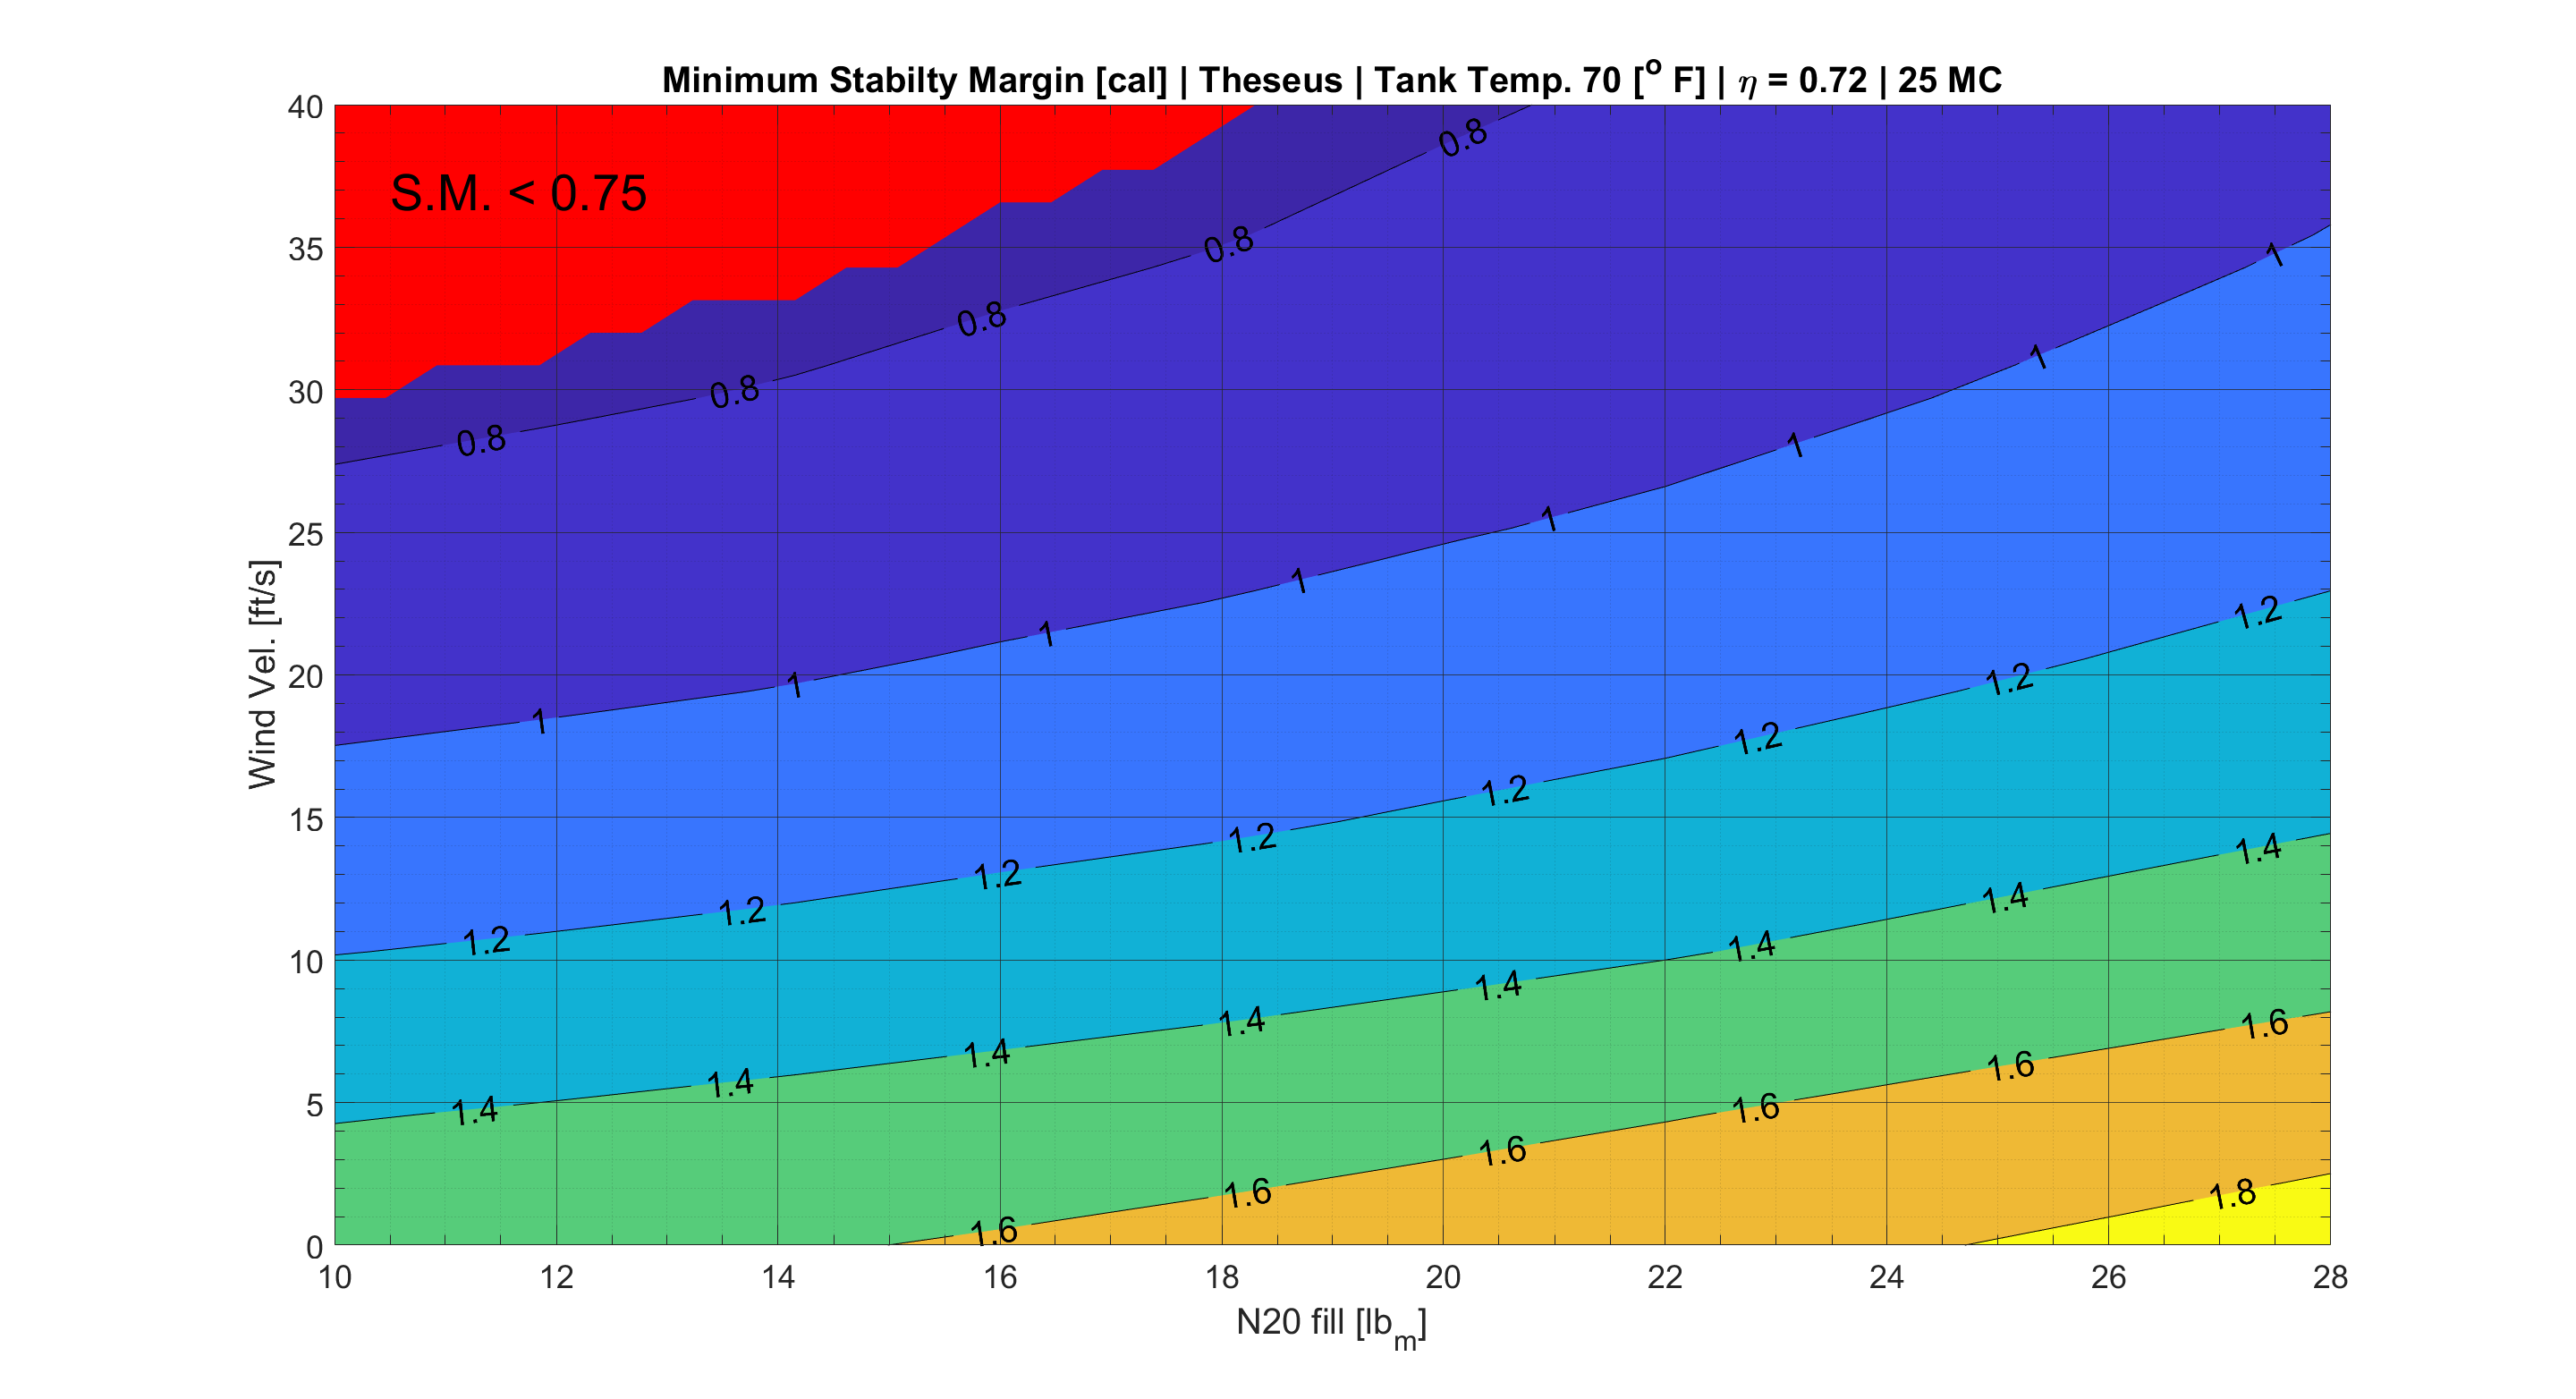
\includegraphics[width=1\textwidth]{./figs/stab_70.png}
 	\caption{Minimum Stability Margin at 70 $^o$ F}
 	\label{fig:stab_70}
 \end{figure}

 \begin{figure}[h!]
	\centering
	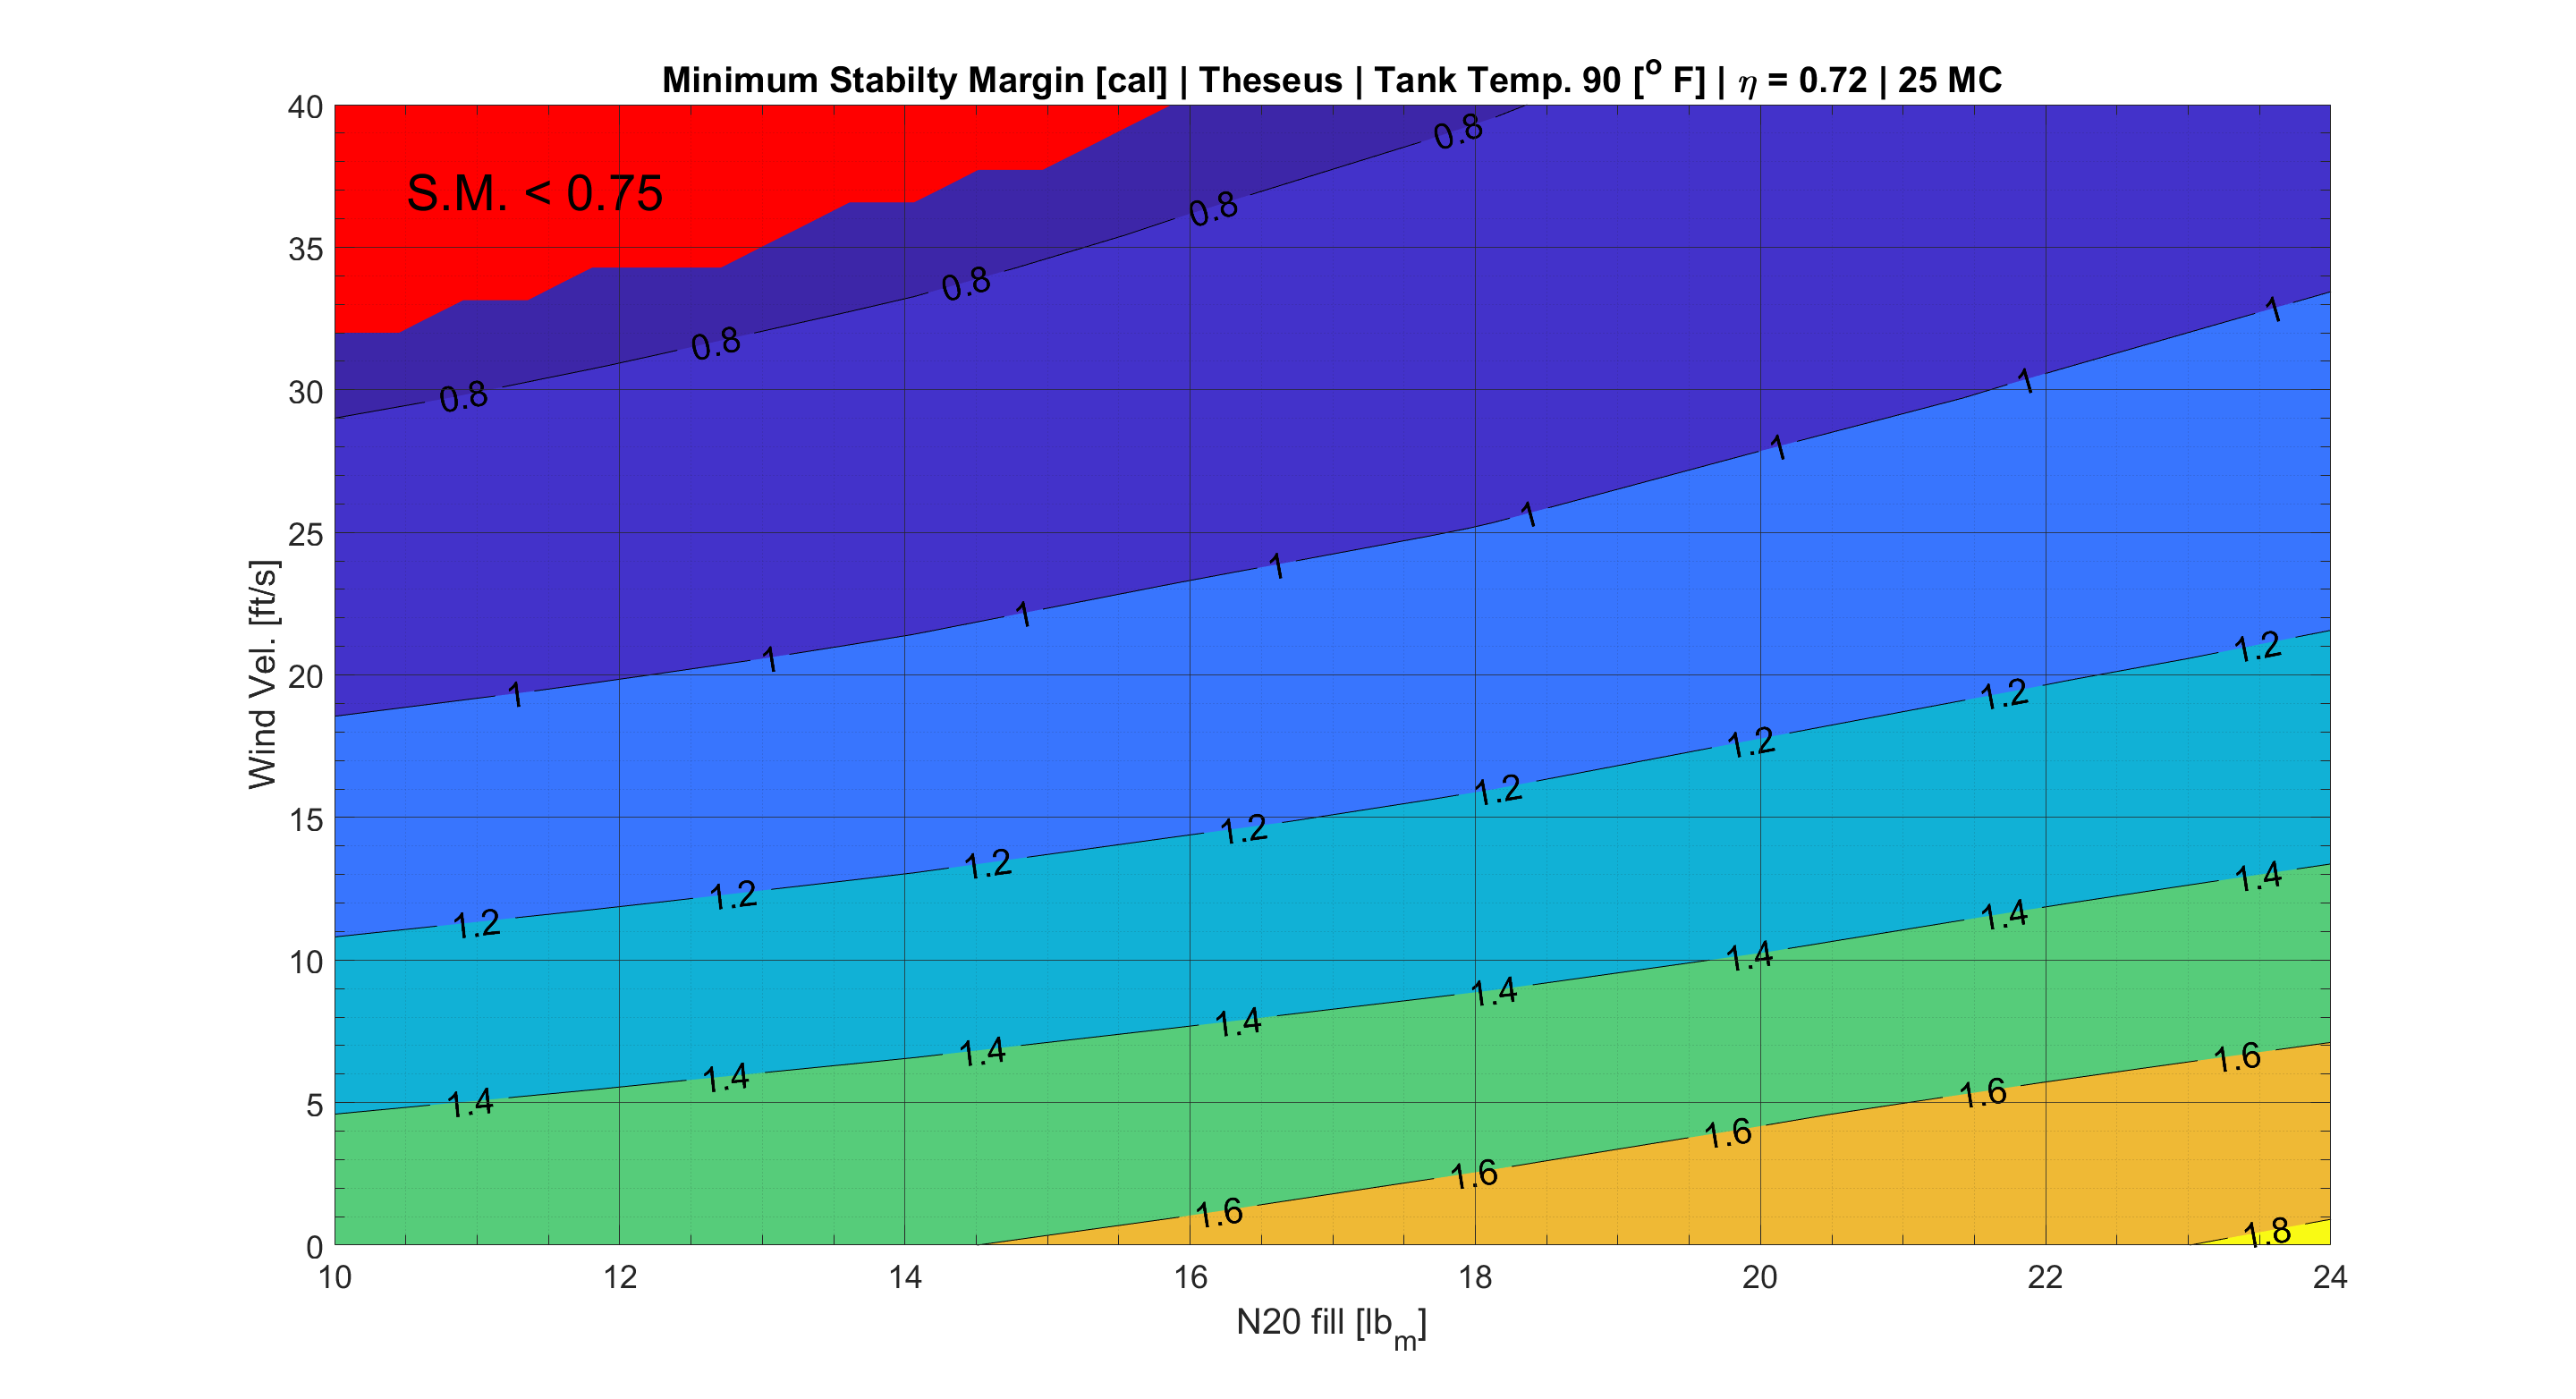
\includegraphics[width=1\textwidth]{./figs/stab_90.png}
	\caption{Minimum Stability Margin at 90 $^o$ F}
	\label{fig:stab_90}
\end{figure}
 
 
 
  
\begin{thebibliography}{10}
	\bibitem{dryden}
	Beal, T.R., 
	"Digital Simulation of Atmospheric Turbulence for Dryden and Von Karman Models,"
	Journal of Guidance, Control, and Dynamics, vol. 16, 1993, pp. 132?138.
	\bibitem{nar}
	National Association of Rocketry,
	"Launching Safely in the 21st Century,"
	Report - Special Committee on Range Operation and Procedure
	\bibitem{monte_carlo}
	Hanson, J.M., and Beard, B.B.,
	"Applying Monte Carlo Simulation to Launch Vehicle Design and Requirements Analysis,"
	NASA/TP - 2010 - 216447, September 2010.
\end{thebibliography}

\end{document}